\documentclass{beamer}
\usetheme{Madrid}

\usepackage{amsmath, amssymb, amsthm}
\usepackage{graphicx}
\usepackage{listings}
\usepackage{gensymb}
\usepackage{minted}
\usemintedstyle{friendly}
\definecolor{bg}{rgb}{0.95,0.95,0.95}
\usepackage[utf8]{inputenc}
\usepackage{hyperref}
\usepackage{gvv}
\begin{document}
\title{NCERT 8 EX-13}
\author{EE24BTECH11032 - JOHN BOBBY}
\date{}
\frame{\titlepage}
\begin{frame}{Question}
\textbf{Question:} Prove that the curves $y^2=4x$ and $x^2=4y$ divide the area of the square bounded by $x=0$,$x=4$,$y=0$,$y=4$ into $3$ equal parts.\\ 
\end{frame}
\begin{frame}{Theoretical Method}
The variables used in $y^2=4x$ are given below
\begin{table}[H]
    \centering
    \begin{tabular}[12pt]{ |c| c| c |}
    \hline
    \textbf{Variable} & \textbf{Description} & \textbf{values}\\ 
    \hline
    $\vec{V}$ & Quadratic form of the matrix & $\myvec{0 & 0 \\ 0 & 1} $\\
    \hline
    $\vec{u}$ & Linear coefficient vector & $\myvec{-2 \\ 0} $\\
    \hline
    f & constant term & 0 \\ 
    \hline
\end{tabular}

\end{table} 
The variables used in $x^2=4y$ are given below
\begin{table}[H]
    \centering
    \begin{tabular}[12pt]{ |c| c| c |}
    \hline
    \textbf{Variable} & \textbf{Description} & \textbf{values}\\ 
    \hline
    $\vec{V}$ & Quadratic form of the matrix & $\myvec{1& 0 \\ 0 & 0} $\\
    \hline
    $\vec{u}$ & Linear coefficient vector & $\myvec{0 \\ -2} $\\
    \hline
    f & constant term & 0 \\ 
    \hline
\end{tabular}

\end{table} 
\end{frame}
\begin{frame}{}
The point of intersection of the line with the parabolas is 
\begin{align}
    x_i = h + k_i m
\end{align}
where, $k_i$ is a constant and is calculated as follows:\\
\begin{align}
k_i = \frac{1}{m^\top Vm} \brak{-m^\top \brak{Vh + u} \pm \sqrt{\sbrak{m^\top \brak{Vh + u}}^2 - g\brak{h}\brak{m^\top Vm}}}.
\end{align}
For line $x=0$ and $y=0$ we get the intersection points with conic  as $\myvec{0 \\0}$ \\
For line $x=4$ and $y=4$ we get the intersection points with conic  as $\myvec{4 \\4}$   
\end{frame}
\begin{frame}{}
Area between $y^2=4x$ and $x^2=4y$ =$\int_{0}^{4} 2\sqrt{x} dx-\int_{0}^{4} \frac{x^2}{4} dx=\frac{32}{3}-\frac{16}{3}=\frac{16}{3}$\\
Area between $x^2=4y$ and $x=0$ and $x=4$=$\int_{0}^{4} 2\sqrt{x} dx=\frac{16}{3}$\\
Area between $y^2=4x$ and $y=0$ and $y=4$ =$\int_{0}^{4} \frac{y^2}{4} dy=\frac{16}{3}$\\
We can see that the $3$ areas are equal.\\
\end{frame}
\begin{frame}{Trapezoidal Method}
Using trapezoidal rule 
\begin{align*}
    \int_{a}^{b} f\brak{x}dx \approx \brak{b-a}\brak{\frac{f\brak{a}+f\brak{b}}{2}}
\end{align*}
Applying trapezoid rule for all values of $x$ between $0$ and $4$\\
where $h$ is the step size 
\begin{align}
    A&=\frac{1}{2}h\brak{y\brak{x_1}+y\brak{x_0}}+ \frac{1}{2}h\brak{y\brak{x_2}+y\brak{x_1}}+\dots+\frac{1}{2}h\brak{y\brak{x_n}+y\brak{x_{n-1}}}
\end{align}
Let $A\brak{x_n}$ be the area enclosed by the curve $y\brak{x}$ from $x=x_0$ to $x=x_n$, $\brak{x_0, x_1, \dots x_n}$ be equidistant points with step-size $h$.
\begin{align}
  A\brak{x_n+h}=A\brak{x_n}+\frac{1}{2}h\brak{y\brak{x_n+h}+y\brak{x_n}}
\end{align}
\end{frame}
\begin{frame}{}
We can repeat this till we get required area.\\
Discretizing the steps, making $A\brak{x_n}=A_n, y\brak{x_n}=y_n$ we get,
\begin{align}
 A_{n+1}=A_n+\frac{1}{2}h\brak{y_{n+1}+y_n}
\end{align}
We can write $y_{n+1}$ in terms of $y_n$ using first principle of derivative. $y_{n+1}=y_n+hy^{\prime}_n$
\begin{align}
  A_{n+1}&=A_n+\frac{1}{2}h\brak{\brak{y_{n}+hy^{\prime}_n}+y_n}\\
  A_{n+1}&=A_n+\frac{1}{2}h\brak{2y_n+hy^{\prime}_n}\\
  A_{n+1}&=A_n+hy_n+\frac{1}{2}h^2y^{\prime}_n\\
  x_{n+1}&=x_n+h
\end{align}
For $y^2=4x$, $y_n=2\sqrt{x_n}$ and $y^{\prime}_n= \frac{1}{\sqrt{x_n}}$\\
For $x^2=4y$, $y_n=\frac{x^2}{4}$ and $y^{\prime}_n= \frac{x}{2}$\\
The general difference equation will be given by
\begin{align}
  A_{n+1}&=A_n+hy_n+\frac{1}{2}h^2y^{\prime}_n\\
  A_{n+1}&=A_n+h\brak{\cos{x_n}}+\frac{1}{2}h^2\brak{-\sin{x_n}}\\
  x_{n+1}&=x_n+h
\end{align}   
\end{frame}
\begin{frame}[fragile]
\frametitle{C-Code}
\begin{minted}[bgcolor=bg, linenos, fontsize=\scriptsize, breaklines]{c}
#include <math.h>
void trapezoidal_1(double *x, double *y, int n, double h) {
    y[0] = 0; 
    for (int i = 0; i < n - 1; i++) {
        y[i+1]=y[i]+h*x[i]*x[i]/4+(h*h*x[i])/4;
    }
}
void trapezoidal_2(double *x, double *y, int n, double h) {
    y[1] = 0; 
    for (int i = 1; i < n - 1; i++) {
        y[i+1]=y[i]+h*2*sqrt(x[i])+(h*h)/(2*sqrt(x[i]));
    }
}
void function_1(double *x,double *y,int n){
	for(int i=0;i<n;i++){
		y[i]=x[i]*x[i]/4;
	}
}
void function_2(double *x,double *y,int n){
	for(int i=0;i<n;i++){
		y[i]=2*sqrt(x[i]);
	}
}
\end{minted}
\end{frame}
\begin{frame}[fragile]
\frametitle{Python-Code}
\begin{minted}[bgcolor=bg, linenos, fontsize=\scriptsize, breaklines]{python}
import numpy as np
import matplotlib.pyplot as plt
import ctypes
# Load the shared library
lib = ctypes.CDLL('./lib.so')
# Set argument and return types for the C functions
lib.trapezoidal_1.argtypes = [ctypes.POINTER(ctypes.c_double), ctypes.POINTER(ctypes.c_double), ctypes.c_int, ctypes.c_double]
lib.trapezoidal_2.argtypes = [ctypes.POINTER(ctypes.c_double), ctypes.POINTER(ctypes.c_double), ctypes.c_int, ctypes.c_double]
lib.function_1.argtypes=[ctypes.POINTER(ctypes.c_double), ctypes.POINTER(ctypes.c_double), ctypes.c_int]
lib.function_2.argtypes=[ctypes.POINTER(ctypes.c_double), ctypes.POINTER(ctypes.c_double), ctypes.c_int]
# Parameters
x_start = 0
x_end = 4
h = 0.1
n_steps = 41

\end{minted}
\end{frame}
\begin{frame}[fragile]
\frametitle{Python-Code}
\begin{minted}[bgcolor=bg, linenos, fontsize=\scriptsize, breaklines]{python}
#Setting up the arrays
area_x = np.linspace(x_start, x_end, n_steps)
area_y_1 = np.zeros(n_steps)
area_y_2 = np.zeros(n_steps)
y_1=np.zeros(n_steps)
y_2=np.zeros(n_steps)
#Conversion to ctypes array
area_x_ctypes = area_x.ctypes.data_as(ctypes.POINTER(ctypes.c_double))
area_y_1_ctypes = area_y_1.ctypes.data_as(ctypes.POINTER(ctypes.c_double))
area_y_2_ctypes = area_y_2.ctypes.data_as(ctypes.POINTER(ctypes.c_double))
y_1_ctypes = y_1.ctypes.data_as(ctypes.POINTER(ctypes.c_double))
y_2_ctypes = y_2.ctypes.data_as(ctypes.POINTER(ctypes.c_double))
# Call the C functions
lib.function_1(area_x_ctypes, y_1_ctypes, n_steps)
lib.trapezoidal_1(area_x_ctypes,area_y_1_ctypes, n_steps,h)
lib.function_2(area_x_ctypes, y_2_ctypes, n_steps)
lib.trapezoidal_2(area_x_ctypes,area_y_2_ctypes, n_steps,h)
#Area variables
Area1=area_y_1[40]
Area2=area_y_2[40]

\end{minted}
\end{frame}
\begin{frame}[fragile]
\frametitle{Python-Code}
\begin{minted}[bgcolor=bg, linenos, fontsize=\scriptsize, breaklines]{python}
# Plotting
plt.figure(figsize=(10, 6))
plt.plot(area_x, y_1, label="Function1", linestyle='-', color='b',linewidth=7)
plt.plot(area_x, y_2, label="Function2", linestyle='-', color='r',linewidth=7)
plt.fill_betweenx(y_2, area_x, np.sqrt(4 * y_2), where=(y_2 >= 0), color='skyblue', alpha=0.5)
plt.fill_between(area_x, y_1, 0, where=(area_x >= 0), color='lightgreen', alpha=0.5)
plt.fill_betweenx(y_2, 0, area_x, where=(y_2 >= 0), color='lightcoral', alpha=0.5)
plt.xlabel("x")
plt.ylabel("y")
#plt.legend()
plt.legend(['$x^2=4y$','$y^2=4x$',f'RegionA(area={Area2-Area1})',f'RegionB(area={Area1})',f'RegionC(area={16-Area2})'])
plt.grid()
#plt.show()
plt.savefig('plot.png')
\end{minted}
\end{frame}
\begin{frame}{Plot}
\begin{figure}[h!]
   \centering
   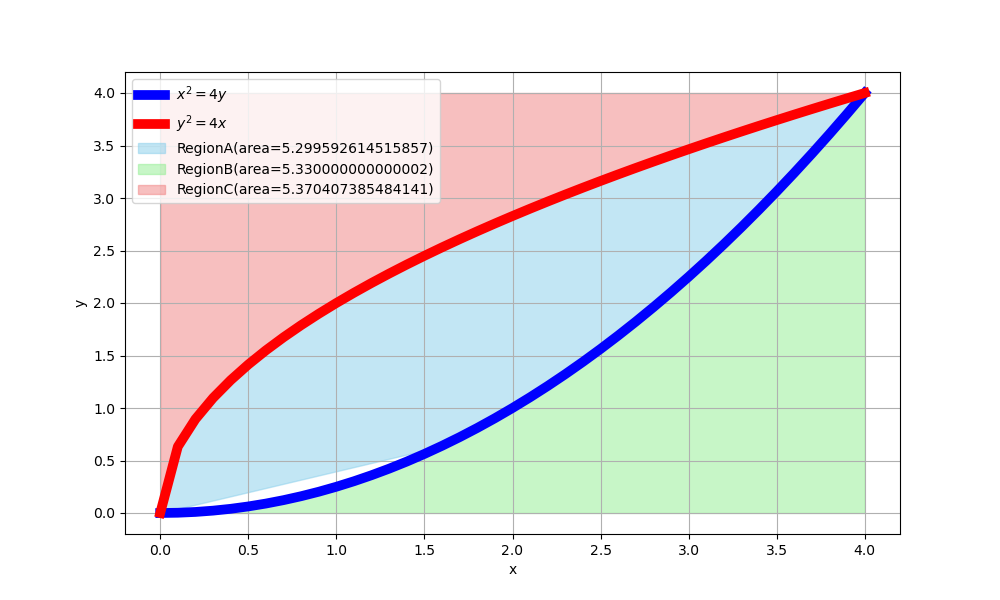
\includegraphics[width=1\columnwidth]{figs/Q3.png}
\end{figure}
    
\end{frame}


\end{document}
